%%%%%%%%%%%%%%%%%%%%%%%%%%%%%%%%%%%%%%%%%%%%%%%%%%%%%%%%%%%
%%%%%%%%%%%%%%%%%%%%%%%%%%%%%%%%%%%%%%%%%%%%%%%%%%%%%%%%%%%
%%%%%%%%%%%%%%%%%%%%%%%%%%%%%%%%%%%%%%%%%%%%%%%%%%%%%%%%%%%

%% PREAMBLE! :-)


\documentclass[a4paper, 10pt]{article} 

%%% packages - input should be path where your packages.tex file is saved.
%% packages

\usepackage{setspace}

%%%%%%%%%%%%%%%%%%%%%%%%%%%%%%%%%%%%%
\usepackage{sectsty}
\usepackage{fontspec}
\setmainfont{STIX Two Text}

\usepackage{lualatex-math}

% \sectionfont{\sffamily\Large}
% \subsectionfont{\sffamily}
%%%%%%%%%%%%%%%%%%%%%%%%%%%%%%%%%%%%%
\usepackage[titles]{tocloft}
%%%%%%%%%%%%%%%%%%%%%%%%%%%%%%%%%%%%%

%%% This is a package to use UTF8 CSV files as input and directly convert them to latex tables.
\usepackage{csvsimple}
%https://texblog.org/2012/05/30/generate-latex-tables-from-csv-files-excel/

%%%%%%%%%%%%%%%%%%%%%%%%%%%%%%%%%%%%%
%%%%%%%%%%%%%%%%%%%%%%%%%%%%%%%%%%%%%
%%%%%%%%%%%%%%%%%%%%%%%%%%%%%%%%%%%%%

\usepackage[version=4]{mhchem}
% package for using chemical equations and fonts 
% https://mirror.kumi.systems/ctan/macros/latex/contrib/mhchem/mhchem.pdf

%%%%%%%%%%%%%%%%%%%%%%%%%%%%%%%%%%%%%
%%%%%%%%%%%%%%%%%%%%%%%%%%%%%%%%%%%%%
%%%%%%%%%%%%%%%%%%%%%%%%%%%%%%%%%%%%%

\usepackage{xparse}
% high level user interface package, use with caution
% https://mirror.easyname.at/ctan/macros/latex/contrib/l3packages/xparse.pdf

%%%%%%%%%%%%%%%%%%%%%%%%%%%%%%%%%%%%%
%%%%%%%%%%%%%%%%%%%%%%%%%%%%%%%%%%%%%
%%%%%%%%%%%%%%%%%%%%%%%%%%%%%%%%%%%%%

\usepackage{makeidx}
\usepackage{pdfpages}
\usepackage{lastpage}

%%%%%%%%%%%%%%%%%%%%%%%%%%%%%%%%%%%%%
%%%%%%%%%%%%%%%%%%%%%%%%%%%%%%%%%%%%%
%%%%%%%%%%%%%%%%%%%%%%%%%%%%%%%%%%%%%

%%% Package to control inclusion and exclusion of specific entry in the table of contents.
%%% https://mirror.foobar.to/CTAN/macros/latex/contrib/tocbibind/tocbibind.pdf
\usepackage[nottoc,notlot,notlof]{tocbibind}

%%%%%%%%%%%%%%%%%%%%%%%%%%%%%%%%%%%%%
%%%%%%%%%%%%%%%%%%%%%%%%%%%%%%%%%%%%%
%%%%%%%%%%%%%%%%%%%%%%%%%%%%%%%%%%%%%

\usepackage{bigstrut}
% needed for crazy table commands, its cool trust me!
% https://anorien.csc.warwick.ac.uk/mirrors/CTAN/macros/latex/contrib/multirow/multirow.pdf

%%%%%%%%%%%%%%%%%%%%%%%%%%%%%%%%%%%%%
%%%%%%%%%%%%%%%%%%%%%%%%%%%%%%%%%%%%%
%%%%%%%%%%%%%%%%%%%%%%%%%%%%%%%%%%%%%

\usepackage{graphicx} 								
% Required for the inclusion of images
% https://de.overleaf.com/learn/latex/Inserting_Images

%%%%%%%%%%%%%%%%%%%%%%%%%%%%%%%%%%%%%
%%%%%%%%%%%%%%%%%%%%%%%%%%%%%%%%%%%%%
%%%%%%%%%%%%%%%%%%%%%%%%%%%%%%%%%%%%%

\usepackage{amsmath} 								
% Required for some math elements 
% https://www.namsu.de/Extra/pakete/amsmath/Amsmath.html

%%%%%%%%%%%%%%%%%%%%%%%%%%%%%%%%%%%%%
%%%%%%%%%%%%%%%%%%%%%%%%%%%%%%%%%%%%%
%%%%%%%%%%%%%%%%%%%%%%%%%%%%%%%%%%%%%

\usepackage{amssymb}
% required for some more crazy math elements, checks mal ab!
% http://milde.users.sourceforge.net/LUCR/Math/mathpackages/amssymb-symbols.pdf

%%%%%%%%%%%%%%%%%%%%%%%%%%%%%%%%%%%%%
%%%%%%%%%%%%%%%%%%%%%%%%%%%%%%%%%%%%%
%%%%%%%%%%%%%%%%%%%%%%%%%%%%%%%%%%%%%

%\usepackage{kbordermatrix} 	
% some special matrix-commands						
% http://www.hss.caltech.edu/~kcb/TeX/kbordermatrix.sty
%%%%%%%%%%%%%%%%%%%%%%%%%%%%%%%%%%%%%
%%%%%%%%%%%%%%%%%%%%%%%%%%%%%%%%%%%%%
%%%%%%%%%%%%%%%%%%%%%%%%%%%%%%%%%%%%%

\usepackage{multicol}								
% multicolumn-commands stuffs
% https://de.overleaf.com/learn/latex/Multiple_columns

%%%%%%%%%%%%%%%%%%%%%%%%%%%%%%%%%%%%%
%%%%%%%%%%%%%%%%%%%%%%%%%%%%%%%%%%%%%
%%%%%%%%%%%%%%%%%%%%%%%%%%%%%%%%%%%%%

\usepackage{color}
\definecolor{dkgreen}{rgb}{0,0.6,0}
\definecolor{gray}{rgb}{0.5,0.5,0.5}
\definecolor{mauve}{rgb}{0.58,0,0.82}
\definecolor{darkblue}{rgb}{0.0,0.0,0.6}
\definecolor{cyan}{rgb}{0.0,0.6,0.6}

%%%%%%%%%%%%%%%%%%%%%%%%%%%%%%%%%%%%%
%%%%%%%%%%%%%%%%%%%%%%%%%%%%%%%%%%%%%
%%%%%%%%%%%%%%%%%%%%%%%%%%%%%%%%%%%%%

% package to more precisely wrap your document around ur figure!
% https://de.overleaf.com/learn/latex/wrapping_text_around_figures
\usepackage{wrapfig}								

%%%%%%%%%%%%%%%%%%%%%%%%%%%%%%%%%%%%%
%%%%%%%%%%%%%%%%%%%%%%%%%%%%%%%%%%%%%
%%%%%%%%%%%%%%%%%%%%%%%%%%%%%%%%%%%%%

% the package for bold math symbol commands!
% https://anorien.csc.warwick.ac.uk/mirrors/CTAN/macros/latex/required/tools/bm.pdf
\usepackage{bm}

%%%%%%%%%%%%%%%%%%%%%%%%%%%%%%%%%%%%%
%%%%%%%%%%%%%%%%%%%%%%%%%%%%%%%%%%%%%
%%%%%%%%%%%%%%%%%%%%%%%%%%%%%%%%%%%%%

% subcaption package dependant on caption package (self-explanatory)
% https://www.namsu.de/Extra/pakete/Subcaption.html

\usepackage{caption}
\usepackage{subcaption}

%%%%%%%%%%%%%%%%%%%%%%%%%%%%%%%%%%%%%
%%%%%%%%%%%%%%%%%%%%%%%%%%%%%%%%%%%%%
%%%%%%%%%%%%%%%%%%%%%%%%%%%%%%%%%%%%%

%package for appendix control
% https://mirror.easyname.at/ctan/macros/latex/contrib/appendix/appendix.pdf
\usepackage[toc,page]{appendix}

%%%%%%%%%%%%%%%%%%%%%%%%%%%%%%%%%%%%%
%%%%%%%%%%%%%%%%%%%%%%%%%%%%%%%%%%%%%
%%%%%%%%%%%%%%%%%%%%%%%%%%%%%%%%%%%%%

% This is the listings package to make code appear like actual code!
% https://mirror.foobar.to/CTAN/macros/latex/contrib/listings/listings.pdf
\usepackage{listings}{
 \lstset{frame=tb,
  basicstyle=\fontsize{8}{10}\selectfont\sffamily,
  frame=single,	 
  language=Python,
  breaklines=true,
  showstringspaces=false,
  columns=flexible,
  numbers=left,
  commentstyle=\color{dkgreen},
  stringstyle=\color{mauve},
  tabsize=2
}

%%%%%%%%%%%%%%%%%%%%%%%%%%%%%%%%%%%%%
%%%%%%%%%%%%%%%%%%%%%%%%%%%%%%%%%%%%%
%%%%%%%%%%%%%%%%%%%%%%%%%%%%%%%%%%%%%

% this package for more elaborate appendix commands!
% http://mirror.ox.ac.uk/sites/ctan.org/macros/latex/contrib/appendix/appendix.pdf
\usepackage[toc,page]{appendix}
%\renewcommand{\appendixpagename}{\appendixname}
%\renewcommand{\appendixtocname}{\appendixname}

%%%%%%%%%%%%%%%%%%%%%%%%%%%%%%%%%%%%%
%%%%%%%%%%%%%%%%%%%%%%%%%%%%%%%%%%%%%
%%%%%%%%%%%%%%%%%%%%%%%%%%%%%%%%%%%%%

% this is the hyperlink references package! To make stuff in your text clickable and send you to the right page, URL's, E-mails etc..
% http://mirror.ox.ac.uk/sites/ctan.org/macros/latex/contrib/hyperref/doc/manual.pdf
\usepackage[
    bookmarks,
    bookmarksopen=true,
    colorlinks=true,			% diese Farbdefinitionen zeichnen Links im PDF farblich aus
    linkcolor=black, 			% einfache interne Verknüpfungen
    anchorcolor=black,			% Ankertext
    citecolor=black, 			% Verweise auf Literaturverzeichniseinträge im Text
    filecolor=magenta, 			% Verknüpfungen, die lokale Dateien öffnen
    menucolor=red, 				% Acrobat-Menüpunkte
    urlcolor=blue,				% URL color of course :P
    plainpages=false,		 	% zur korrekten Erstellung der Bookmarks
    pdfpagelabels, 				% zur korrekten Erstellung der Bookmarks
    hypertexnames=true, 		% zur korrekten Erstellung der Bookmarks
    %linktocpage 				% Seitenzahlen anstatt Text im Inhaltsverzeichnis verlinken
]{hyperref}

\usepackage{tcolorbox}
%Fancy boxes around text!
%%%%%%%%%%%%%%%%%%%%%%%%%%%%%%%%%%%%%

\usepackage{amsthm}
\usepackage{algorithm}
\usepackage{algpseudocode}
\usepackage{tikz} 

%%% Settings!
%% settings
%change relevant macros like title, names etc.

\newcommand{\firstauthorfirstname}{Camilo }
\newcommand{\firstauthorlastname}{Tello Fachin }

\newcommand{\secondauthorfirstname}{Tobias }
\newcommand{\secondauthorlastname}{Sloviak }

\newcommand{\doctitle}{Programming Project 2}

\makeindex
%%%%%%%%%%%%%%%%%%%%%%%%%%%%%%%%%%%%%%%%%%%%%%%%%%%%%%%%%%%%%%%%%%%%%%%%%
%%%%%%%%%%%%%%%%%%%%%%%%%%%%%%%%%%%%%%%%%%%%%%%%%%%%%%%%%%%%%%%%%%%%%%%%%
%%%%%%%%%%%%%%%%%%%%%%%%%%%%%%%%%%%%%%%%%%%%%%%%%%%%%%%%%%%%%%%%%%%%%%%%%

% set the margins of the document, single first input generates evenly spaced margins of that value
\usepackage[margin=2.5cm]{geometry}

%%%%%%%%%%%%%%%%%%%%%%%%%%%%%%%%%%%%%%%%%%%%%%%%%%%%%%%%%%%%%%%%%%%%%%%%%
%%%%%%%%%%%%%%%%%%%%%%%%%%%%%%%%%%%%%%%%%%%%%%%%%%%%%%%%%%%%%%%%%%%%%%%%%
%%%%%%%%%%%%%%%%%%%%%%%%%%%%%%%%%%%%%%%%%%%%%%%%%%%%%%%%%%%%%%%%%%%%%%%%%

\usepackage[utf8]{inputenc}
% u need this one to compile ä ö ü while babel-package is disabled!(english document)!!
% https://www.namsu.de/Extra/pakete/Inputenc.html

%\usepackage[ngerman]{babel}
% uncomment this package to have all the generated text lik TOC and TOC-APP in german
% IF U UNCOMMENT THIS, PUT THE UTF8 INPUTENC PACKAGE IN COMMENT
% https://www.namsu.de/Extra/pakete/German.html

%%%%%%%%%%%%%%%%%%%%%%%%%%%%%%%%%%%%%%%%%%%%%%%%%%%%%%%%%%%%%%%%%%%%%%%%%
%%%%%%%%%%%%%%%%%%%%%%%%%%%%%%%%%%%%%%%%%%%%%%%%%%%%%%%%%%%%%%%%%%%%%%%%%
%%%%%%%%%%%%%%%%%%%%%%%%%%%%%%%%%%%%%%%%%%%%%%%%%%%%%%%%%%%%%%%%%%%%%%%%%


% header and footer settings
% to look up stuff on it go visit this one:
% https://en.wikibooks.org/wiki/LaTeX/Customizing_Page_Headers_and_Footers

\usepackage{fancyhdr}
\setlength{\headheight}{22.25pt}

\renewcommand{\headrulewidth}{0.5pt}
\renewcommand{\footrulewidth}{0.5pt}

\pagestyle{fancy}


% header inputs
\lhead[even output]{HOT}
\chead[even output]{Programming Project 2}
\rhead[even output]{
\includegraphics[width=2.5cm]{figures/uni_header}}


%footer inputs
\lfoot[even output]{CSE - WS23}
\cfoot[even output]{Page  \thepage}
\rfoot[even output]{\today}

%%%%%%%%%%%%%%%%%%%%%%%%%%%%%%%%%%%%%%%%%%%%%%%%%%%%%%%%%%%%%%%%%%%%%%%%%
%%%%%%%%%%%%%%%%%%%%%%%%%%%%%%%%%%%%%%%%%%%%%%%%%%%%%%%%%%%%%%%%%%%%%%%%%
%%%%%%%%%%%%%%%%%%%%%%%%%%%%%%%%%%%%%%%%%%%%%%%%%%%%%%%%%%%%%%%%%%%%%%%%%


%settings for PDF metadata, available if rightclick on pdf in adobe and chose properties!

\hypersetup{pdfinfo={
Title={\doctitle},
Subject={Heuristic Optimization Techniques},
Author={Camilo Tello Fachin, Tobias Sloviak},
Keywords={Combinatorial Optimization, }{Julia, }{S-Plex, }{Winter Semester 2023, }
{MSc Computational Science and Engineering, }{TU Vienna}
}}

%%%%%%%%%%%%%%%%%%%%%%%%%%%%%%%%%%%%%%%%%%%%%%%%%%%%%%%%%%%%%%%%%%%%%%%%%
%%%%%%%%%%%%%%%%%%%%%%%%%%%%%%%%%%%%%%%%%%%%%%%%%%%%%%%%%%%%%%%%%%%%%%%%%
%%%%%%%%%%%%%%%%%%%%%%%%%%%%%%%%%%%%%%%%%%%%%%%%%%%%%%%%%%%%%%%%%%%%%%%%%

%% This is the bibliography package,
\usepackage[
backend=bibtex,
style=ieee,
sorting=ynt,
backref=false,
hyperref=true
]{biblatex}

%%%%%%%%%%%%%%%%%%%%%%%%%%%%%%%%%%%%%%%%%%%%%%%%%%%%%%%%%%%%%%%%%%%%%%%%%
%%%%%%%%%%%%%%%%%%%%%%%%%%%%%%%%%%%%%%%%%%%%%%%%%%%%%%%%%%%%%%%%%%%%%%%%%
%%%%%%%%%%%%%%%%%%%%%%%%%%%%%%%%%%%%%%%%%%%%%%%%%%%%%%%%%%%%%%%%%%%%%%%%%

%%% This is an important setting which lets u control the spacing between lines! Just comment/uncomment the desired ones!


%\singlespacing

\onehalfspacing

%\doublespacing

%%%%%%%%%%%%%%%%%%%%%%%%%%%%%%%%%%%%%%%%%%%%%%%%%%%%%%%%%%%%%%%%%%%%%%%%%

%%% custom commands

\newcommand{\var}[1]{\texttt{#1}}
\newcommand{\fun}[1]{\texttt{#1}}
\newcommand{\obj}[1]{\texttt{#1}}
\newcommand{\MPIRD}[0]{\texttt{MPI\_Reduce}}
\newcommand{\MPIBC}[0]{\texttt{MPI\_Bcast}}
\newcommand{\MPI}[0]{\texttt{MPI} }

\newtheorem*{theorem*}{Theorem}
\newtheorem*{proof*}{Proof} 

%%% macros - where u define ur macros and newcommands!
% useful macros!


% insert a blank page which is still counted
\newcommand{\blankpage}{
\newpage
\thispagestyle{empty}
\mbox{}
\newpage
}

%%% the bibliohraphy! the settings to the bibliography are changed in the packages.tex file, where the bibtex package is loaded!
\addbibresource{content/04_bibliography.bib}

\begin{document}


%%%%%%%%%%%%%%%%%%%%%%%%%%%%%%%%%%%%%%%%%%%%%%%%%%%%%%%%%%%
%%%%%%%%%%%%%%%%%%%%%%%%%%%%%%%%%%%%%%%%%%%%%%%%%%%%%%%%%%%%
%%%%%%%%%%%%%%%%%%%%%%%%%%%%%%%%%%%%%%%%%%%%%%%%%%%%%%%%%%%
          

\begin{titlepage}

\newcommand{\HRule}{\rule{\linewidth}{0.5mm}} % Defines a new command for the horizontal lines, change thickness here

\center % Center everything on the page
 
%----------------------------------------------------------------------------------------
%	HEADING SECTIONS
%----------------------------------------------------------------------------------------

\textsc{\LARGE Vienna University of Technology}\\[1.5cm] % Name of your university/college
\textsc{\Large 192.137 Heuristic Optimization Techniques}\\[0.5cm] % Major heading such as course name
\textsc{\large TU Wien Algorithmics and Complexity Group}\\[0.5cm] % Minor heading such as course title

%----------------------------------------------------------------------------------------
%	TITLE SECTION
%----------------------------------------------------------------------------------------

\HRule \\[0.5cm]
{ \huge \bfseries \doctitle}\\[1mm] % Title of your document
\HRule \\[0.5cm]
 
%----------------------------------------------------------------------------------------
%	AUTHOR SECTION
%----------------------------------------------------------------------------------------
\hfill

\begin{minipage}{0.58\textwidth}
\begin{flushleft} \large
\emph{Authors:}\\
\null
Tobias \textsc{Sloviak}\\
01204691 \\
\null
Camilo \textsc{Tello Fachin}\\
12127084 \\

\end{flushleft}
\end{minipage}
~
\begin{minipage}{0.4\textwidth}
\begin{flushleft} \large
\emph{Supervisors:} \\
\null
Prof. Dr. Günther \textsc{Raidl} \\ % Supervisor's Name
\null
Dipl. Ing. Enrico \textsc{Iurlano} \\ % Supervisor's Name
\null
Dipl. Ing. Laurenz \textsc{Tomandl} \\ % Supervisor's Name
\null
\end{flushleft}
\end{minipage}\\[1.5cm]
\hfill

% If you don't want a supervisor, uncomment the two lines below and remove the section above
%\Large \emph{Author:}\\
%John \textsc{Smith}\\[3cm] % Your name

%----------------------------------------------------------------------------------------
%	DATE SECTION
%----------------------------------------------------------------------------------------
\vfill
\null

{\large \today}\\[1cm] % Date, change the \today to a set date if you want to be precise

%----------------------------------------------------------------------------------------
%	LOGO SECTION 
%----------------------------------------------------------------------------------------



\includegraphics[width=0.75\textwidth]{figures/uni_titlepage}\\ % Include a department/university logo
 
%----------------------------------------------------------------------------------------

\vfill % Fill the rest of the page with whitespace
\pagenumbering{alph}

\end{titlepage} 

%\blankpage

% this is to remove the first paragraph sentence indentation! if you want indentation, set the second input to the desired indendation value.
\setlength{\parindent}{0pt}

% this file is loaded, to include PDF's such as declaration of intent for theses, abstracts and summaries in other languages.
\pagenumbering{roman}

% \section*{Abstract}
% Here documented the results of exercise 2, the Programming part of High Performance Computing.
% A presentation for Marco Schmid MSc.



%%% If your TOC is too large for one page, you can distribute it over 2 pages and comment this /blankpage command below! To better control the distribution of the content of the table of content, use the geometry settings and adjust the top and bottom margin for the table of content in the next part of this code.

%\blankpage



%%% Here u define the TOC, a newgeometry command is used to let you design your own TOC margins. just comment out the \newgeometry and the \restoregeometry
%%% command to force the same margins as the rest of the document to the TOC

\pagebreak
\thispagestyle{empty}
\newgeometry{top=2.25cm, bottom=2.25cm}
{\sffamily\tableofcontents}
\thispagestyle{empty}
\restoregeometry
\pagebreak

\pagenumbering{arabic}


%%%%%%%%%%%%%%%%%%%%%%%%%%%%%%%%%%%%%%%%%%%%%%%%%%%%%%%%%%%
%%%%%%%%%%%%%%%%%%%%%%%%%%%%%%%%%%%%%%%%%%%%%%%%%%%%%%%%%%%
%%%%%%%%%%%%%%%%%%%%%%%%%%%%%%%%%%%%%%%%%%%%%%%%%%%%%%%%%%%
%%%%%%%%%%%%%%%%%%%%%%%%%%%%%%%%%%%%%%%%%%%%%%%%%%%%%%%%%%%



%%% This is a first surrogate chapter to intuitively show you how and where to include new chapters!asd
\section*{To Do's}
\begin{itemize}
    \item either make framework work or create new framework
    \item analyze locks in lecture slides and in paper:
    \item \begin{itemize}
        \item Test-and-Set Lock
        \item Test-and-Test-and-Set Lock
        \item Ticket Lock
        \item Array Lock
        \item CLH Lock
        \item MCS Lock
        \item Hemlock (from paper..)
    \end{itemize}
    \item in the lectureslides from the project it says:
    \item \begin{itemize}
        \item Benchmark the following two under various scenarious, meaning low/high contention 
        \item Benchmark Throughput (probably locks-unlocks performed per time)
        \item Benchmark Latency 
        \item Benchmark for fairness, we have to think of some number to measure fairness, maybe locks/unlocks achieved per thread
    \end{itemize}
\end{itemize}
\pagebreak





%\pagebreak

\section{Introduction}

\begin{proof*}
    let $X \in [C^{0,1}(\bar{\Omega})]^2$ with $X \rvert_{\Gamma_{\infty}} = 0$ be a given vectorfield. \\
    Set $\mathrm{T}_t(.) := \mathrm{id} + tX $ , with $t \in \mathbb{R}$ and $\Omega_t := \mathrm{T}_t(\Omega)$, where 
    $(\mathbf{u}_t, p_t)$ solve this and $\Omega$ is replaced by $\Omega_t$ s.t. \\
    $p_t \in \mathrm{L}^2(\Omega_t), \int_{\Omega_t} p_t \, \mathrm{dx} = 0 $ and $\mathrm{u}_t \in [H^1(\Omega_t)]^2$. Then there holds 
    \begin{align}
        \int_{\Omega_t} \mathrm{D} \mathbf{u}_t : \mathrm{D} \mathbf{\mathbf{v}} + \mathrm{div}(\mathbf{v}) \, p_t + \mathrm{div}(\mathbf{u}_t) \, q \, dx = \, 0 \quad \forall (v,q)
        \in  [H^1_0(\Omega_t)]^d \times L^2(\Omega_t).
    \end{align}
    Introduction of change of variables shows that $(\mathbf{u}^t, p^t) := (\mathbf{u}_t \circ \mathrm{T}_t, p_t \circ \mathrm{T}_t)$ satisfy
    \begin{equation}
    \begin{aligned}\label{trafo_weak_stokes}
        &\int_\Omega \mathrm{det}(\mathrm{DT}_t)
        \left( \mathrm{DT}_t^{-1} \mathrm{D}\mathbf{u}^t:\mathrm{DT}_t^{-1} \mathrm{D}\mathbf{v} -p\, \mathrm{tr}(\mathrm{D}\mathbf{v}\mathrm{DT}_t^{-1})  +
        q \, \mathrm{tr}(\mathrm{D}\mathbf{u}\mathrm{DT}_t^{-1}) \right) \mathrm{dx}, \\
        & \quad \quad \quad \quad \quad \quad \quad \quad \quad \ \forall (v,q) \in [H^1(\Omega)]^2 \times L^2(\Omega),
    \end{aligned}
    \end{equation}
    Used in equation (\ref{trafo_weak_stokes})
    \begin{align*}
        \mathrm{D}\mathbf{v}\circ\mathrm{T}_t &= \mathrm{D}(\mathbf{v}\circ\mathrm{T}_t), \\
        \mathrm{div}(\mathbf{v}) &= \mathrm{tr} \left( \mathrm{D}(\mathbf{v} \circ \mathrm{T}_t)(\mathrm{DT}_t^{-1}) \right).
    \end{align*}
      
    The functional $J(\Omega,\mathbf{u})$ is now reduced to the functional $J(\Omega)$, since the change of the quantities $(\mathbf{u},p)$
    is taken into account by the transformation theorem. The minimum of (\ref{energy_dissipation_equation})
    satisfies the saddlepoint problem . It can be obtained with the Lagrange Multiplier method, 
    see Faustmann . The corresponding Lagrangian which can be used to minimize is
    \begin{equation}\label{parametrized_lagrangian}
     \begin{aligned}
        \mathcal{L}(t,\mathbf{v}, q) = \frac{1}{2}& \int_{\Omega} \mathrm{det}(\mathrm{DT}_t) \mathrm{D} \mathbf{v}(\mathrm{DT}_t)^{-1} :
        \mathrm{D} \mathbf{v}(\mathrm{DT}_t)^{-1} \, \mathrm{dx}, \\
        &- \int_{\Omega}\mathrm{det}(\mathrm{DT}_t)q \, \mathrm{tr} \left( \mathrm{D}\mathbf{v}(\mathrm{DT}_t)^{-1} \right).
    \end{aligned}
    \end{equation}
    To find the shape derivative, one can now derive this parametrized Lagrangian, for details on the derivation of parametrized Lagrangians, 
    see K. Ito et. al. . With the derivative of the Lagrangian obtained, it holds true that
    \begin{align}
        \mathrm{d}J(\Omega)(X) =\ \frac{\mathrm{d}}{\mathrm{d}t} \mathcal{L}(t, \mathbf{u}^t, 0)\big\rvert_{t=0}  =
        \frac{\partial}{\partial t}\mathcal{L}(0,\mathbf{u},p) = \int_{\Omega} \mathrm{S}_1 : \mathrm{D}X \, \mathrm{dx}.
    \end{align}
    \qed
    \end{proof*}

\pagebreak

\section{Questions}

\textcolor{red}{
In the end, here will be the answer to the question "Think about a meaningful real-world application for this problem and briefly describe it."\\
1. Think about a meaningful real-world application for this problem and briefly describe it.\\
2. Develop a meaningful deterministic construction heuristic.\\
3. Derive a randomized construction heuristic to be applied iteratively.\\
4. Develop or make use of a framework for basic local search which is able to deal with:\\
• different neighborhood structures\\
• different step functions (first-improvement, best-improvement, random)\\
5. Develop a set of meaningful neighborhood structures to address the different aspects of the problem,
i.e., related to the quality of the s-plexes, or the assignment of nodes to s-plexes.\\
6. Develop or make use of a Variable Neighborhood Descent (VND) framework which uses your
neighborhood structures.\\
7. Implement a Greedy Randomized Adaptive Search Procedure (GRASP) using your randomized
construction heuristic and an effective neighborhood structure with one step function or (a vari-
ant of) your VND. Note that the union of existing neighborhood structures also constitutes a
(composite) neighborhood structure.\\
8. Implement one of the following metaheuristics:\\
• General Variable Neighborhood Search (GVNS) on top of your VND\\
• Simulated Annealing (SA)\\
• Tabu Search (TS)\\
9. Perform some manual tuning of relevant algorithmic parameters to find sensible parameter settings
for the final experiments. Relevant parameters may be related to the degree of randomization,
neighborhood structure sizes, probabilities for the random step function in composite neighborhood
structures, the cooling schedule, the tabu list length and its variation, etc. Report the impact of a
number of different settings on the solution quality of a selected meaningful subset of instances.
10. Use delta-evaluation.\\
Explain which steps in your algorithm use delta-evaluation and describe
why delta-evaluation results in better performance in this step. Are there other elements in your
algorithm that could have also benefitted from delta-evaluation?\\
11. Run experiments and compare all your algorithms on the instances provided in TUWEL:\\
(a) deterministic and randomized construction heuristic and GRASP\\
(b) Use the solution of the deterministic construction heuristic to test the other implementations:\\
i. Local search for at least three selected (possibly composite) neighborhood structures using
each of the three step functions (i.e., at least nine different algorithm variants).\\
ii. VND\\
iii. GVNS, SA, or TS\\
12. Write a report containing the description of your algorithms, the experimental results and what
you conclude from them; see the general information document for more details.}

\pagebreak

\section{Questions to Consider during developtment}

\textcolor{red}{
• How is your solution represented?\\
• Ad 4: How do you generate different solutions? Which parts of your algorithm can be reasonably
randomized and how can you control the degree of randomization?\\
• Ad 3 and 4: Does randomization and iterated application improve the generated solutions?\\
• What parameters do you use and which values do you chose for them?\\
• Can subsequent – possibly non-improving – moves in your neighborhood structures reach every\\
solution in the search space? Or at least one optimal solution?
• Local search: How many iterations does it take on average to reach a local optima? What does
this say about your neighborhood structures?\\
• How does incremental evaluation work for your neighborhood structures?\\
• What is the time complexity to fully search one neighborhood of your neighborhood structures?\\
• VND: Does the order of your neighborhood structures affect the solution quality?}

\pagebreak

\section{Real World application}

A general s-plex application that is probably used is the identification of group or friend networks
where one can make assumptions about group or friend networks. This is application is not directly
derived from our programming assignment, but it is somewhat related since one still has to identify k-plexes in a
undirected graph which with the amount of people using social media these days is not trivial.
An application that is closer to the given s-plex programming assignment would be telecommunication networks.
Where the distance between the antennas, towers or compute node could be correlated to the weight matrix and the s-plex
relaxation of the clique's could be used to make crucial system more reduntant (low s-plexes) and other less crucial systems
less reduntant (higher s-plexes).

\section{Deterministic Construction Heuristic}

Our first idea for a construction of solutions is the following: An empty graph (without edges) is always 
a 1-plex, since a single node without edges is a 1-plex. Removing all the edges gives a valid solution, 
however a very bad one. Our first idea for an algorithm that finds a good solution was to start with an 
empty graph and go through all the edges in $A_0$, check if adding them to $A$ is legal and if so, do that. 
This algorithm improves the empty graph, however it can only find $s$-plexes of up to $|S|=s+1$. The reason 
is that it will connect the first node $v_1$ with $\min(s,\deg_{A_0} (v_1))$ many other nodes, then the 
cluster of $v_1$ is an $s$-plex with size at most $s+1$ and no more nodes can be added. Then, all the other 
nodes in the cluster might get connected among each other, but the $s$-plex will not get any bigger. 
Practically speaking, with this construction we got approximately $n/(s+1)$ many clusters of size $s+1$ 
which were mostly fully connected, so this construction results in small clusters.\\

\textcolor{red}{
deterministic construction heuristic where we explain how the construction heuristic is done.
Maybe only do on the problem with 9 vertices and plot some results.}

\pagebreak

\section{Randomized Construction Heuristic}

For our random construction we randomly parse the entries of $A_0$ but do the same as above otherwise.

\subsection{Local improvement move operators}
After this point we found it difficult to think of the next move, because simply adding one edge in this state 
will always yield an illegal solution. In trying to understand the problem better, we wrote the adjacency 
matrices $A_0$ in files and looked at their structure. What we found was that there is a structure in most of the 
graphs, more precisely there are 3 types of graphs (see also figure \ref{fig:types}):

\begin{enumerate}
    \item locally strongly connected: 26/60 (Here, nodes that are close in numbering are also strongly connected 
    in the graph)
    \item seemingly randomly connected: 23/60
    \item tentacle-like connected: 7/60 (Here, the Graphs have a semi-large, strongly 
    connected cluster with "tentacles" reaching out. Tentacle-shaped clusters are bad for $s$-plexes, 
    so we will have to seperate these "lines" into small "spheres".)
\end{enumerate}

\begin{figure}[h]
\centering
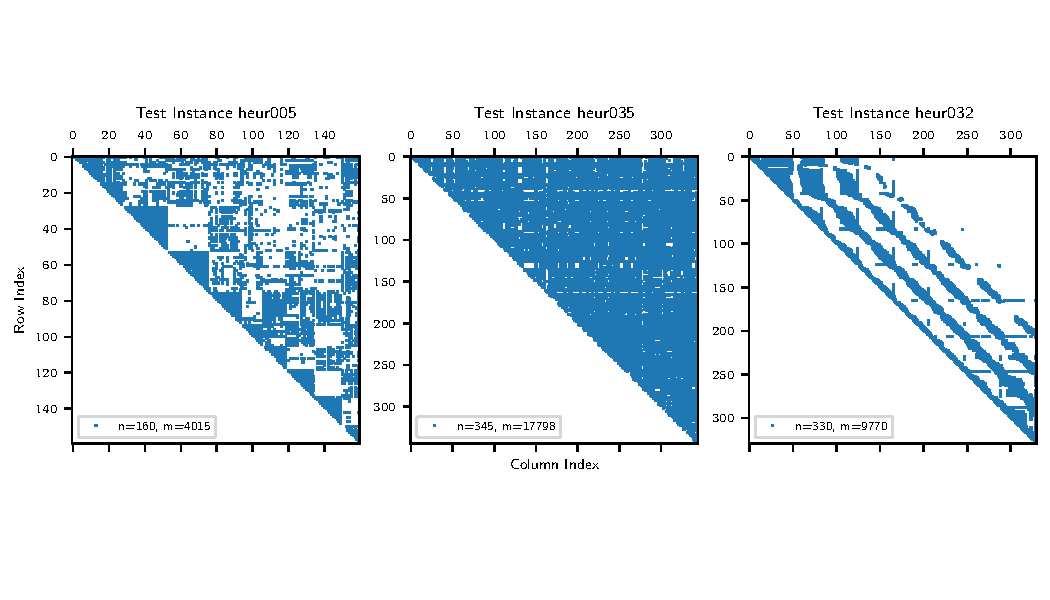
\includegraphics[width=\linewidth, trim= {0 1.8cm 0 1.8cm}, clip]{figures/spy_adjacency.pdf}
\caption{\label{fig:types}Instances of the different graph types. Left is a locally strongly 
connected graph, this is part of instance 005. In the middle is a seemingly randomly connected graph, 
which is part of instance 035. On the right is a tentacle-like connected graph, which is part of instance 032.}
\end{figure}

We will use this special structure of some instances to derive parts of our algorithms. Some might consider 
this cheating, but we think, that finding patterns in the instances is an important part of solving problems 
in real world applications so we find it to be okay. We will see later, that for the locally strongly connected 
instances we can find reasonably good solutions with very little computational effort. We will also see that 
the algorithms that were derived with the locally connected graphs in mind also work well on the other graphs.\\



\pagebreak



\pagebreak

\section{Neighborhood Structures and Step Functions}

\textcolor{red}{
Develop or make use of a framework for basic local search which is able to deal with: \\
• different neighborhood structures\\
• different step functions (first-improvement, best-improvement, random)\\
5. Develop a set of meaningful neighborhood structures to address the different aspects of the problem,
i.e., related to the quality of the s-plexes, or the assignment of nodes to s-plexes.}

\pagebreak

\section{Variable Neighborhood Descent (VNS)}
text

\pagebreak

\section{Greedy Randomized Adaptive Search Procedure (GRASP)}

\pagebreak

\section{Exercise 5 - Integrated, Improved Binary Tree Algorithm}


\pagebreak

\section{Manual Paramter Tuning}
\textcolor{red}{
Perform some manual tuning of relevant algorithmic parameters to find sensible parameter settings
for the final experiments. Relevant parameters may be related to the degree of randomization,
neighborhood structure sizes, probabilities for the random step function in composite neighborhood
structures, the cooling schedule, the tabu list length and its variation, etc. Report the impact of a
number of different settings on the solution quality of a selected meaningful subset of instances.}

\pagebreak

\section{Delta Evaluation}
\textcolor{red}{Use delta-evaluation.
Explain which steps in your algorithm use delta-evaluation and describe
why delta-evaluation results in better performance in this step. Are there other elements in your
algorithm that could have also benefitted from delta-evaluation?}

\pagebreak

\section{Chapter 7}

\pagebreak

\section{Results and Conclusion}

\textcolor{red}{
Run experiments and compare all your algorithms on the instances provided in TUWEL:\\
(a) deterministic and randomized construction heuristic and GRASP\\
(b) Use the solution of the deterministic construction heuristic to test the other implementations:\\
i. Local search for at least three selected (possibly composite) neighborhood structures using
each of the three step functions (i.e., at least nine different algorithm variants).\\
ii. VND\\
iii. GVNS, SA, or TS}
%%%%%%%%%%%%%%%%%%%%%%%%%%%%%%%%%%%%%%%%%%%%%%%%%%%%%%%%%%%
%%%%%%%%%%%%%%%%%%%%%%%%%%%%%%%%%%%%%%%%%%%%%%%%%%%%%%%%%%%
%%%%%%%%%%%%%%%%%%%%%%%%%%%%%%%%%%%%%%%%%%%%%%%%%%%%%%%%%%%
%%%%%%%%%%%%%%%%%%%%%%%%%%%%%%%%%%%%%%%%%%%%%%%%%%%%%%%%%%%


%% During the document writing process, this single .tex file is used to let dasdyou write down a little to do list, just comment it out when the paper is done!

%%%%%%%%%%%%%%%%%%%%%%%%%%%%%%%%%%%%%%%%%%%%%%%%%%%%%%%%%%%
%%%%%%%%%%%%%%%%%%%%%%%%%%%%%%%%%%%%%%%%%%%%%%%%%%%%%%%%%%%
%%%%%%%%%%%%%%%%%%%%%%%%%%%%%%%%%%%%%%%%%%%%%%%%%%%%%%%%%%%
%%%%%%%%%%%%%%%%%%%%%%%%%%%%%%%%%%%%%%%%%%%%%%%%%%%%%%%%%

%%% Bibliography printing at this point! 
\addcontentsline{toc}{section}{References}
\printbibliography

%%% This is a hardcoded string to enforce it in the table of contents, if you want your "references" string in the TOC to be named differently, such as bibliography or so on, just change the third input to this command below to your desired references naming that should appear in the TOC



\pagebreak

%%%%%%%%%%%%%%%%%%%%%%%%%%%%%%%%%%%%%%%%%%%%%%%%%%%%%%%%%%%
%%%%%%%%%%%%%%%%%%%%%%%%%%%%%%%%%%%%%%%%%%%%%%%%%%%%%%%%%%%
%%%%%%%%%%%%%%%%%%%%%%%%%%%%%%%%%%%%%%%%%%%%%%%%%%%%%%%%%%%


%%% This is where the appendix .tex file is included, the settings to the appendix are changed in the settings.tex file
%\begin{appendix}
\addappheadtotoc
\section{CPP CUDA Code - Strided and Offset Memory Access - Task 1a}
\label{app_1a}

\begin{lstlisting}[language=C++, title=C++ Listing for EX1 a)]
#include <stdio.h>
#include "timer.hpp"
#include <algorithm>
#include <vector>

__global__ void addVec_kth(double *x, double *y, double *z, int N, int k) {
	unsigned int total_threads = blockDim.x * gridDim.x;
	unsigned int global_tid = blockIdx.x * blockDim.x + threadIdx.x;
	if (k==0) {
		k = 1;
	}
	for (unsigned int i = global_tid; i<N/k; i += total_threads) {
		z[i*k] = x[i*k] + y[i*k];
	}
}

// findMedian function for any vector lenghts, source geeksforgeeks.com
double findMedian(std::vector<double> a,
                  int n)
{
    if (n % 2 == 0) {
        std::nth_element(a.begin(),
                    a.begin() + n / 2,
                    a.end());
        std::nth_element(a.begin(),
                    a.begin() + (n - 1) / 2,
                    a.end());
        return (double)(a[(n - 1) / 2]
                        + a[n / 2])
               / 2.0;
    }
    else {
        std::nth_element(a.begin(),
                    a.begin() + n / 2,
                    a.end());
        return (double)a[n / 2];
    }
}

int main(void)
{
	// Task 1a//
	double *x, *y, *z, *gpu_x, *gpu_y, *gpu_z;
	double eff_BW;
	Timer timer;
	int N = pow(10.0, 8.0);
	std::vector<int> k_values(64, 0);
	for(int i = 0; i<64; i++){
		k_values[i] = i;
	}
	std::vector<double> exec_timings = {0, 0, 0, 0, 0, 0, 0, 0, 0, 0, 0};
	x = (double*)malloc(N*sizeof(double));
	y = (double*)malloc(N*sizeof(double));
	z = (double*)malloc(N*sizeof(double));
	for (int i = 0; i < N; i++) {
		x[i] = (double)(i);
		y[i] = (double)(N-i-1);
	}
	cudaMalloc(&gpu_x, N*sizeof(double)); 
	cudaMalloc(&gpu_y, N*sizeof(double));
	cudaMalloc(&gpu_z, N*sizeof(double));
	cudaMemcpy(gpu_x, x, N*sizeof(double), cudaMemcpyHostToDevice);
	cudaMemcpy(gpu_y, y, N*sizeof(double), cudaMemcpyHostToDevice);
	cudaMemcpy(z, gpu_z, N*sizeof(double), cudaMemcpyDeviceToHost);

	for (int i = 0; i < 64; i++) {
		for (int m = 0; m < 11; m++) {
			timer.reset();
			addVec_kth<<<256, 256>>>(gpu_x, gpu_y, gpu_z, N, k_values[i]);
			cudaDeviceSynchronize();
			exec_timings[m] = timer.get();
		}
		if (k_values[i]==0) {
			eff_BW = 3 * N * sizeof(double) * pow(10,-9) / findMedian(exec_timings, 10);
		}
		else{
			eff_BW = 3 * floor((N/k_values[i])) * sizeof(double) * pow(10, -9) / findMedian(exec_timings, 10);
		}
		printf("%d,%g\n", k_values[i], eff_BW);
	}

	cudaFree(gpu_x);
	cudaFree(gpu_y);
	cudaFree(gpu_z);
	free(x);
	free(y);
	free(z);
\end{lstlisting}
\pagebreak

\section{CPP CUDA Code - Offset Memory Access - Task 1b}
The code for the Offset Memory Access partial exercise is the same as for the
Strided Memory Access partial exercise, except the \texttt{\_\_global\_\_} part where
the offset is defined and the calculation of the effective bandwidth, where one can now
 also omit the case distinction for k=0.

\null

\label{app_1b}
\begin{lstlisting}[language=C++, title=C++ Listing for EX1 b)]
__global__ void addVec_kth(double *x, double *y, double *z, int N, int k) {
	unsigned int total_threads = blockDim.x * gridDim.x;
	unsigned int global_tid = blockIdx.x * blockDim.x + threadIdx.x;
	if (k==0) {
		k = 1;
	}
	for (unsigned int i = global_tid; i<N-k; i += total_threads) {
		z[i+k] = x[i+k] + y[i+k];
	}
}

.
.
.

eff_BW = 3 * floor((N - k_values[i])) * sizeof(double) * pow(10, -9) / findMedian(exec_timings, 10);

.
.
.

\end{lstlisting}

\pagebreak

\section{CPP CUDA Code - Dense Matrix Transpose - Task 2b}
\label{app_2b}

\begin{lstlisting}[language=C++, title=C++ Listing for EX2 b and c]
#include <stdio.h>
#include <iostream>
#include "timer.hpp"
#include "cuda_errchk.hpp"   // for error checking of CUDA calls

__global__
void transpose(double *A, double *B, int N)
{
  int t_idx = blockIdx.x*blockDim.x + threadIdx.x;
  int row_idx = t_idx / N;
  int col_idx = t_idx % N;
  
  if (row_idx < N && col_idx < N) B[row_idx * N + col_idx] = A[col_idx * N + row_idx];
}


void print_A(double *A, int N)
{
  for (int i = 0; i < N; i++) {
    for (int j = 0; j < N; ++j) {
      std::cout << A[i * N + j] << ", ";
    }
    std::cout << std::endl;
  }
}

int main(void)
{
  int N = 10;

  double *A, *cuda_A, *B, *cuda_B;
  Timer timer;

  // Allocate host memory and initialize
  A = (double*)malloc(N*N*sizeof(double));
  B = (double*)malloc(N*N*sizeof(double));
  
  for (int i = 0; i < N*N; i++) {
    A[i] = i;
  }

  print_A(A, N);


  // Allocate device memory and copy host data over
  CUDA_ERRCHK(cudaMalloc(&cuda_A, N*N*sizeof(double))); 
  CUDA_ERRCHK(cudaMalloc(&cuda_B, N*N*sizeof(double))); 

  // copy data over
  CUDA_ERRCHK(cudaMemcpy(cuda_A, A, N*N*sizeof(double), cudaMemcpyHostToDevice));

  // wait for previous operations to finish, then start timings
  CUDA_ERRCHK(cudaDeviceSynchronize());
  timer.reset();

  // Perform the transpose operation
  transpose<<<(N*N+255)/256, 256>>>(cuda_A, cuda_B, N);

  // wait for kernel to finish, then print elapsed time
  CUDA_ERRCHK(cudaDeviceSynchronize());
  double elapsed = timer.get();
  std::cout << std::endl << "Time for transpose: " << elapsed << std::endl;
  std::cout << "Effective bandwidth: " << (2*N*N*sizeof(double)) / elapsed * 1e-9 << " GB/sec" << std::endl;
  std::cout << std::endl;

  // copy data back (implicit synchronization point)
  CUDA_ERRCHK(cudaMemcpy(B, cuda_B, N*N*sizeof(double), cudaMemcpyDeviceToHost));

  print_A(B, N);

  cudaFree(cuda_A);
  cudaFree(cuda_B);
  free(A);
  free(B);

  CUDA_ERRCHK(cudaDeviceReset());  // for CUDA leak checker to work

  return EXIT_SUCCESS;
}
\end{lstlisting}


\end{appendix}



%%%%%%%%%%%%%%%%%%%%%%%%%%%%%%%%%%%%%%%%%%%%%%%%%%%%%%%%%%%
%%%%%%%%%%%%%%%%%%%%%%%%%%%%%%%%%%%%%%%%%%%%%%%%%%%%%%%%%%%
%%%%%%%%%%%%%%%%%%%%%%%%%%%%%%%%%%%%%%%%%%%%%%%%%%%%%%%%%%%


\end{document}

